\chapter{Módulos Especializados}

\begin{figure}[H]
	\centering
	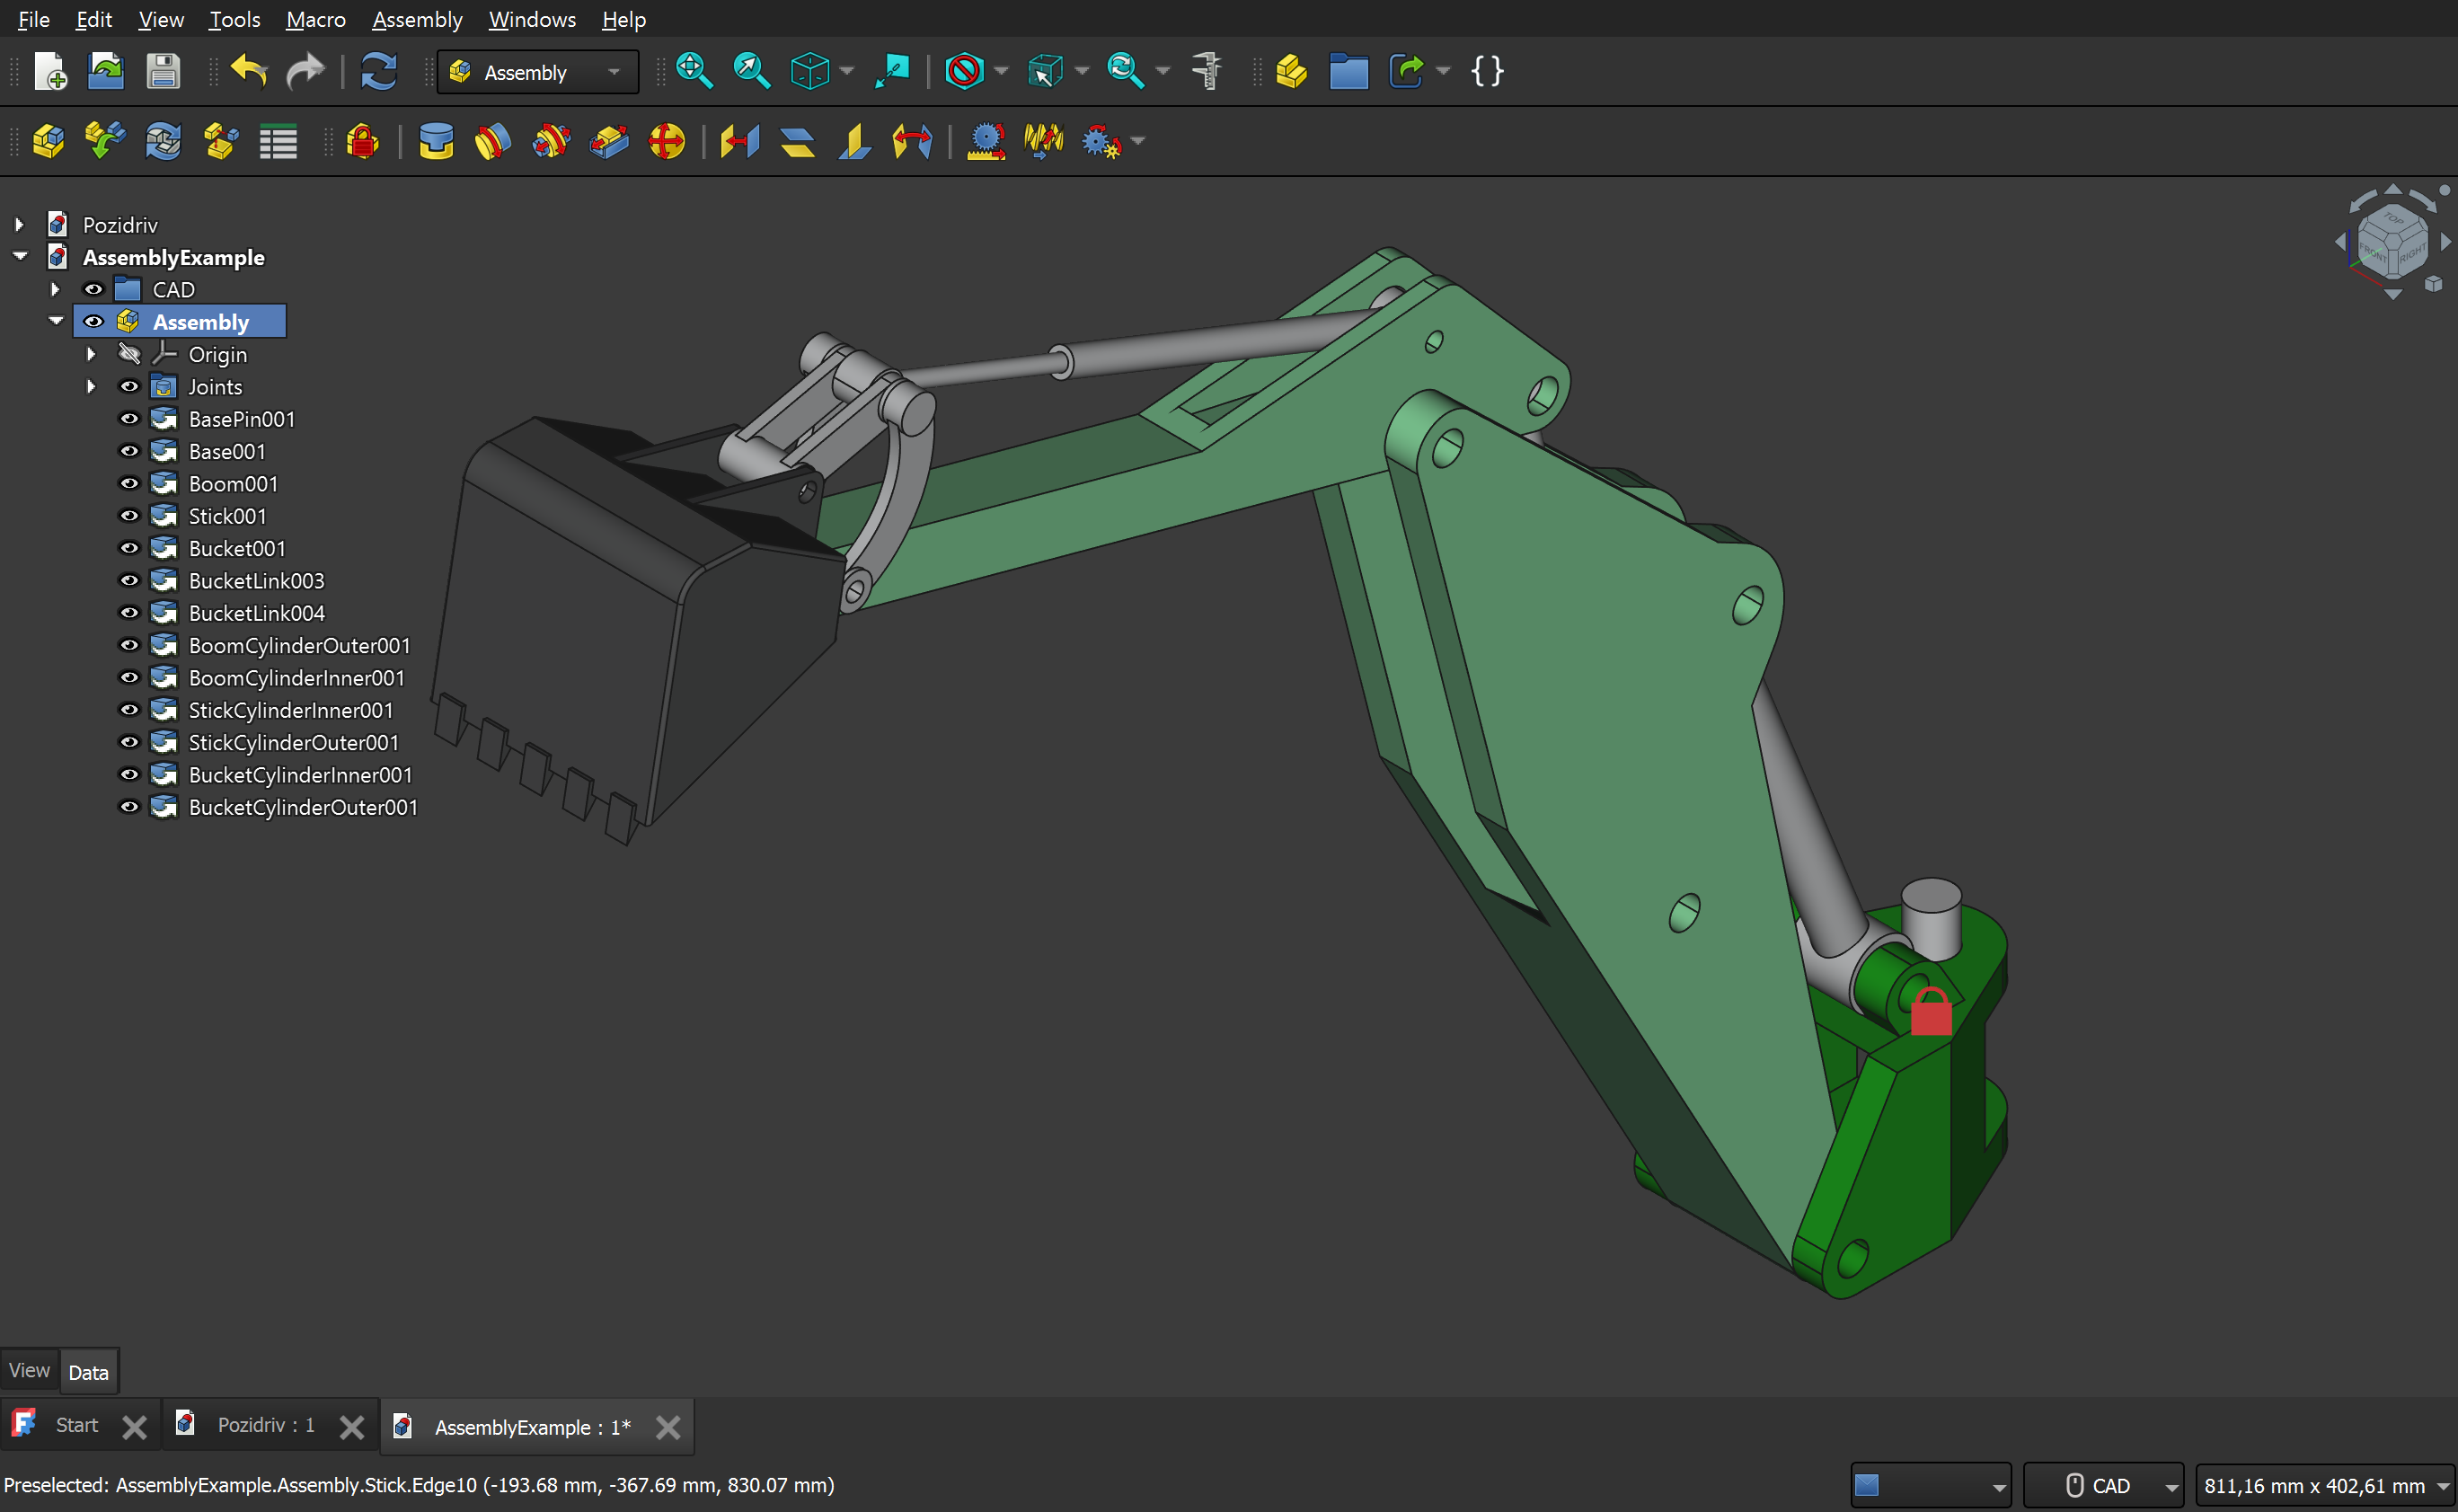
\includegraphics[width=0.8\textwidth]{img/cap7_modulos.png}
	\caption{Módulos especializados de FreeCAD en acción}
\end{figure}

Conoce los módulos especializados de FreeCAD: Part
Design, Sketcher, Draft y otros. Cada módulo está
diseñado para tareas específicas de diseño.

%% D. Búsqueda e Inserción de Activos Gráficos
%% Imagen insertada al inicio del capítulo

%% B. Actividades Teóricas
\section{Investigar y responder}
\faPencil

Investiga sobre módulos de FreeCAD y responde:
\begin{enumerate}
	\item ¿Cuál es la diferencia entre Part y Part Design?
	\item ¿Qué funciones específicas tiene el módulo Sketcher?
	\item ¿Para qué sirve el módulo Draft en FreeCAD?
	\item ¿Qué ventajas ofrece el módulo Arch para
	      arquitectura?
	\item ¿Cómo se cambia entre diferentes workbenches?
	\item ¿Qué módulos son esenciales para diseño mecánico?
	\item ¿Cómo se instalan módulos adicionales o plugins?
	\item ¿Qué módulos son recomendados para principiantes?
\end{enumerate}

%% C. Actividades Prácticas
\section{Resolver los siguientes problemas}
\faWrench

Problemas para aplicar conocimientos:
\begin{enumerate}
	\item Explora el módulo Part Design y crea una pieza
	      simple.
	\item Usa el módulo Sketcher para crear un boceto
	      complejo con restricciones.
	\item Trabaja con el módulo Draft para crear geometría
	      2D con proyección a 3D.
	\item Explora el módulo Arch y crea una pared simple.
	\item Compara las herramientas de Part y Part Design
	      para la misma tarea.
	\item Crea una pieza usando el flujo de trabajo de
	      Part Design.
	\item Instala un módulo adicional desde el administrador
	      de complementos.
	\item Personaliza tu barra de herramientas con accesos
	      directos a módulos.
	\item Crea un archivo que combine herramientas de
	      múltiples módulos.
	\item Documenta las diferencias entre al menos tres
	      módulos de FreeCAD.
\end{enumerate}